%!TEX root =../../course-notes.tex
% ^ leave for LaTeXTools build functionality

\begin{applicationActivities}{3}{27}

\begin{activity}{5}
  Suppose the matrix \(M\) is invertable, so there exists \(M^{-1}\)
  with \(MM^{-1}=I\). It follows that \(\det(M)\det(M^{-1})=\det(I)\).

  What is the only number that \(\det(M)\) cannot equal?
  \begin{multicols}{4}
  \begin{enumerate}[(a)]
  \item \(-1\)
  \item \(0\)
  \item \(1\)
  \item \(\frac{1}{\det(M^{-1})}\)
  \end{enumerate}
  \end{multicols}
\end{activity}

\begin{fact}
  Since \(\det(M^{-1})=\frac{1}{\det(M)}\) for every invertable matrix \(M\),
  a square matrix \(M\) is invertable if and only if \(\det(M)\not=0\).
\end{fact}

\begin{observation}
Consider the linear transformation $A : \IR^2 \rightarrow \IR^2$ given by the matrix $A = \begin{bmatrix} 2 & 2 \\ 0 & 3 \end{bmatrix}$

\begin{center}
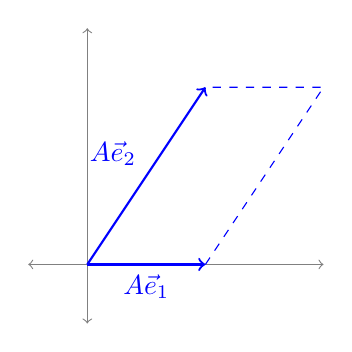
\begin{tikzpicture}[scale=0.75]
\draw[thin,gray,<->] (-1,0)-- (4,0);
\draw[thin,gray,<->] (0,-1)-- (0,4);
\draw[thick,blue,->] (0,0) -- node[below] {$A \vec{e}_1$}++ (2,0);
\draw[thick,blue,->] (0,0) -- node[above left] {$A \vec{e}_2$}++(2,3);
\draw[blue,dashed] (2,0) -- (4,3) -- (2,3);
\end{tikzpicture}
\end{center}
It is easy to see geometrically that  $$ A\begin{bmatrix}1 \\ 0 \end{bmatrix} = \begin{bmatrix}2 \\ 0 \end{bmatrix}= 2 \begin{bmatrix}1 \\ 0 \end{bmatrix}$$

It is less obvious (but easily verified by computation) that
$$A\begin{bmatrix} 2 \\ 1 \end{bmatrix} = \begin{bmatrix} 6 \\ 3 \end{bmatrix} = 3\begin{bmatrix} 2 \\ 1 \end{bmatrix}$$
\end{observation}

\begin{definition}Let $A \in \IR^{n \times n}$.
An \term{eigenvector} is a vector $\vec{x} \in \IR^n$ such that $A\vec{x}$ is parallel to $\vec{x}$.

In other words, $A\vec{x}=\lambda \vec{x}$ for some scalar $\lambda$.
We call this \(\lambda\) an \term{eigenvalue} of \(A\).
\end{definition}

\begin{observation}
Since \(\lambda\vec x=\lambda (I\vec x)\), we can find the eigenvalues and
eigenvectors satisfying $A\vec{x}=\lambda \vec{x}$ by inspecting
$(A-\lambda I)\vec{x} = \vec0$.
\begin{itemize}
\item Since we already know that $(A-\lambda I)\vec0 = \vec0$
for any value of \(\lambda\),
we are more interested in finding values of $\lambda$ such that
$A-\lambda I$ has a nontrivial kernel.
\item Thus \(\RREF(A-\lambda I)\) must have a non-pivot column, and therefore
\(A-\lambda I\) cannot be invertable.
\item
Since \(A-\lambda I\) cannot be invertable, our eigenvalues must satisfy
\(\det(A-\lambda I)=0\).
\end{itemize}
\end{observation}

\begin{definition}
Computing \(\det(A-\lambda I)\) results in the
\term{characteristic polynomial} of \(A\).

For example, when
\(A=\begin{bmatrix}1 & 2 \\ 3 & 4\end{bmatrix}\), we have

\[
  A-\lambda I=
  \begin{bmatrix}1 & 2 \\ 3 & 4\end{bmatrix}-
  \begin{bmatrix}\lambda & 0 \\ 0 & \lambda\end{bmatrix}=
  \begin{bmatrix}1-\lambda & 2 \\ 3 & 4-\lambda\end{bmatrix}
\]

Thus the characteristic polynomial of \(A\) is

\[
  \det\begin{bmatrix}1-\lambda & 2 \\ 3 & 4-\lambda\end{bmatrix}
=
  (1-\lambda)(4-\lambda)-6
=
  \lambda^2-5\lambda-2
\]
% Computing $\det(A-\lambda I)$ is called the \term{characteristic polynomial} of $A$.  It is a polynomial in the variable $\lambda$.
% \item Once an eigenvalue is found, the eigenvectors form a subspace called the \term{eigenspace}, which is simply the kernel of $A-\lambda I$.  Each eigenvalue will have an associated eigenspace.
\end{definition}

\begin{activity}{15}
  Complete the following computation of the characteristic polynomial
  \(A-\lambda I\) for
  $A=\begin{bmatrix} 6 & -2 & 1 \\ 17 & -5 & 5 \\ -4 & 2 & 1 \end{bmatrix}$.

  \scalebox{.8}{\parbox{1.2\linewidth}{
  \begin{align*}
    \begin{bmatrix} 6-\lambda & -2 & 1 \\ 17 & -5-\lambda & 5 \\ -4 & 2 & 1-\lambda \end{bmatrix}
  &=
    (6-\lambda)\det \begin{bmatrix}
      \unknown & \unknown & \unknown \\
      0 & 1 & -1 \\
      1 & 2 & 0
    \end{bmatrix}
    -2\det \begin{bmatrix}
      \unknown & \unknown & \unknown \\
      0 & 1 & -1 \\
      1 & 2 & 0
    \end{bmatrix}
    +\det \begin{bmatrix}
      \unknown & \unknown & \unknown \\
      0 & 1 & -1 \\
      1 & 2 & 0
    \end{bmatrix}
  \\ &=
    (6-\lambda)\det \begin{bmatrix}
      1 & 0 & 0 \\
      \unknown & \unknown & \unknown \\
      \unknown & \unknown & \unknown \\
    \end{bmatrix}
    +2\det \begin{bmatrix}
      1 & 0 & 0 \\
      \unknown & \unknown & \unknown \\
      \unknown & \unknown & \unknown \\
    \end{bmatrix}
    -\det \begin{bmatrix}
      1 & 0 & 0 \\
      \unknown & \unknown & \unknown \\
      \unknown & \unknown & \unknown \\
    \end{bmatrix}
  \\ &=
    (6-\lambda)\det \begin{bmatrix}
      \unknown & \unknown \\
      \unknown & \unknown \\
    \end{bmatrix}
    +2\det \begin{bmatrix}
      \unknown & \unknown \\
      \unknown & \unknown \\
    \end{bmatrix}
    -\det \begin{bmatrix}
      \unknown & \unknown \\
      \unknown & \unknown \\
    \end{bmatrix}
  \\ &=
    (6-\lambda)((-5-\lambda)(1-\lambda)-10)
    +2(17(1-\lambda)+20)
    -(-4(-5-\lambda)-34)
  \end{align*}}}
\end{activity}

\begin{activity}{15}
Let $A = \begin{bmatrix} 2 & 2 \\ 0 & 3 \end{bmatrix}$.
\begin{subactivity}
Compute $\det \begin{bmatrix} 2-\lambda & 2 \\ 0 & 3-\lambda \end{bmatrix}$ to determine the characteristic polynomial of $A$.
\end{subactivity}
\begin{subactivity}
Find the roots of the characteristic polynomial
to determine the eigenvalues of $A$.
\end{subactivity}
\begin{subactivity}
Compute the kernel of the transformation given by
\[
  A-2I
    =
  \begin{bmatrix} 2-2 & 2 \\ 0 & 3-2 \end{bmatrix}
\] to determine all the eigenvectors associated to the eigenvalue $2$.
\end{subactivity}
\begin{subactivity}
Compute the kernel of the transformation given by $A-3I$ to determine all the eigenvectors associated to the eigenvalue $3$.
\end{subactivity}
\end{activity}

\begin{definition}
  The kernel of the transformation given by \(A-\lambda I\) contains
  all the eigenvectors associated with \(\lambda\). Since kernel is a subspace
  of \(\IR^n\), we call this kernel the \term{eigenspace} associated with the
  eigenvalue \(\lambda\).
\end{definition}


\begin{activity}{15}
  Find all the eigenvalues and associated eigenspaces for the matrix $A=\begin{bmatrix} 3 & -2 & 1 \\  0 & 2 & 8 \\ 0 & 2 & 2 \end{bmatrix}$.

\begin{subactivity}
 Compute $\det (A-\lambda I)$ to determine the characteristic polynomial of $A$.
\end{subactivity}
\begin{subactivity}
Find the roots of the characteristic polynomial
\((3-\lambda)(\lambda^2-4\lambda-12)\)
to determine the eigenvalues of $A$.
\end{subactivity}
\begin{subactivity}
Compute the kernels of $A-\lambda I$ for each eigenvalue
$\lambda\in\{-2,3,6\}$ to determine the respective eigenspaces.
\end{subactivity}
\end{activity}

\end{applicationActivities}
